\documentclass[twoside]{book}

% Packages required by doxygen
\usepackage{fixltx2e}
\usepackage{calc}
\usepackage{doxygen}
\usepackage[export]{adjustbox} % also loads graphicx
\usepackage{graphicx}
\usepackage[utf8]{inputenc}
\usepackage{makeidx}
\usepackage{multicol}
\usepackage{multirow}
\PassOptionsToPackage{warn}{textcomp}
\usepackage{textcomp}
\usepackage[nointegrals]{wasysym}
\usepackage[table]{xcolor}

% Font selection
\usepackage[T1]{fontenc}
\usepackage[scaled=.90]{helvet}
\usepackage{courier}
\usepackage{amssymb}
\usepackage{sectsty}
\renewcommand{\familydefault}{\sfdefault}
\allsectionsfont{%
  \fontseries{bc}\selectfont%
  \color{darkgray}%
}
\renewcommand{\DoxyLabelFont}{%
  \fontseries{bc}\selectfont%
  \color{darkgray}%
}
\newcommand{\+}{\discretionary{\mbox{\scriptsize$\hookleftarrow$}}{}{}}

% Page & text layout
\usepackage{geometry}
\geometry{%
  a4paper,%
  top=2.5cm,%
  bottom=2.5cm,%
  left=2.5cm,%
  right=2.5cm%
}
\tolerance=750
\hfuzz=15pt
\hbadness=750
\setlength{\emergencystretch}{15pt}
\setlength{\parindent}{0cm}
\setlength{\parskip}{3ex plus 2ex minus 2ex}
\makeatletter
\renewcommand{\paragraph}{%
  \@startsection{paragraph}{4}{0ex}{-1.0ex}{1.0ex}{%
    \normalfont\normalsize\bfseries\SS@parafont%
  }%
}
\renewcommand{\subparagraph}{%
  \@startsection{subparagraph}{5}{0ex}{-1.0ex}{1.0ex}{%
    \normalfont\normalsize\bfseries\SS@subparafont%
  }%
}
\makeatother

% Headers & footers
\usepackage{fancyhdr}
\pagestyle{fancyplain}
\fancyhead[LE]{\fancyplain{}{\bfseries\thepage}}
\fancyhead[CE]{\fancyplain{}{}}
\fancyhead[RE]{\fancyplain{}{\bfseries\leftmark}}
\fancyhead[LO]{\fancyplain{}{\bfseries\rightmark}}
\fancyhead[CO]{\fancyplain{}{}}
\fancyhead[RO]{\fancyplain{}{\bfseries\thepage}}
\fancyfoot[LE]{\fancyplain{}{}}
\fancyfoot[CE]{\fancyplain{}{}}
\fancyfoot[RE]{\fancyplain{}{\bfseries\scriptsize Generated by Doxygen }}
\fancyfoot[LO]{\fancyplain{}{\bfseries\scriptsize Generated by Doxygen }}
\fancyfoot[CO]{\fancyplain{}{}}
\fancyfoot[RO]{\fancyplain{}{}}
\renewcommand{\footrulewidth}{0.4pt}
\renewcommand{\chaptermark}[1]{%
  \markboth{#1}{}%
}
\renewcommand{\sectionmark}[1]{%
  \markright{\thesection\ #1}%
}

% Indices & bibliography
\usepackage{natbib}
\usepackage[titles]{tocloft}
\setcounter{tocdepth}{3}
\setcounter{secnumdepth}{5}
\makeindex

% Hyperlinks (required, but should be loaded last)
\usepackage{ifpdf}
\ifpdf
  \usepackage[pdftex,pagebackref=true]{hyperref}
\else
  \usepackage[ps2pdf,pagebackref=true]{hyperref}
\fi
\hypersetup{%
  colorlinks=true,%
  linkcolor=blue,%
  citecolor=blue,%
  unicode%
}

% Custom commands
\newcommand{\clearemptydoublepage}{%
  \newpage{\pagestyle{empty}\cleardoublepage}%
}

\usepackage{caption}
\captionsetup{labelsep=space,justification=centering,font={bf},singlelinecheck=off,skip=4pt,position=top}

%===== C O N T E N T S =====

\begin{document}

% Titlepage & ToC
\hypersetup{pageanchor=false,
             bookmarksnumbered=true,
             pdfencoding=unicode
            }
\pagenumbering{alph}
\begin{titlepage}
\vspace*{7cm}
\begin{center}%
{\Large \textquotesingle{}cpp\textquotesingle{} }\\
\vspace*{1cm}
{\large Generated by Doxygen 1.8.13}\\
\end{center}
\end{titlepage}
\clearemptydoublepage
\pagenumbering{roman}
\tableofcontents
\clearemptydoublepage
\pagenumbering{arabic}
\hypersetup{pageanchor=true}

%--- Begin generated contents ---
\chapter{Hierarchical Index}
\section{Class Hierarchy}
This inheritance list is sorted roughly, but not completely, alphabetically\+:\begin{DoxyCompactList}
\item \contentsline{section}{figure}{\pageref{classfigure}}{}
\begin{DoxyCompactList}
\item \contentsline{section}{disque}{\pageref{classdisque}}{}
\item \contentsline{section}{rectangle}{\pageref{classrectangle}}{}
\item \contentsline{section}{triangle}{\pageref{classtriangle}}{}
\end{DoxyCompactList}
\end{DoxyCompactList}

\chapter{Class Index}
\section{Class List}
Here are the classes, structs, unions and interfaces with brief descriptions\+:\begin{DoxyCompactList}
\item\contentsline{section}{\hyperlink{classdisque}{disque} }{\pageref{classdisque}}{}
\item\contentsline{section}{\hyperlink{classfigure}{figure} }{\pageref{classfigure}}{}
\item\contentsline{section}{\hyperlink{classrectangle}{rectangle} }{\pageref{classrectangle}}{}
\item\contentsline{section}{\hyperlink{classtriangle}{triangle} }{\pageref{classtriangle}}{}
\end{DoxyCompactList}

\chapter{Class Documentation}
\hypertarget{classdisque}{}\section{disque Class Reference}
\label{classdisque}\index{disque@{disque}}


{\ttfamily \#include $<$disque.\+h$>$}



Inheritance diagram for disque\+:
\nopagebreak
\begin{figure}[H]
\begin{center}
\leavevmode
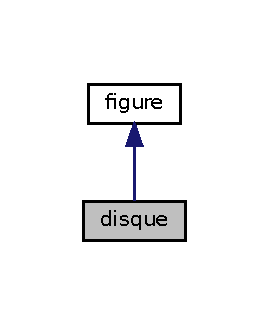
\includegraphics[width=129pt]{classdisque__inherit__graph}
\end{center}
\end{figure}


Collaboration diagram for disque\+:
\nopagebreak
\begin{figure}[H]
\begin{center}
\leavevmode
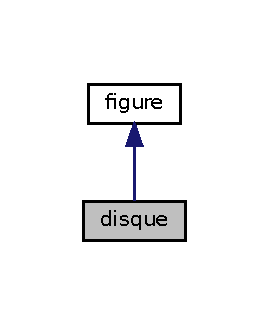
\includegraphics[width=129pt]{classdisque__coll__graph}
\end{center}
\end{figure}
\subsection*{Public Member Functions}
\begin{DoxyCompactItemize}
\item 
double \hyperlink{classdisque_a050ca11b1180244c645b4122a8a675a5}{perimetre} (double pi, double rayon)
\item 
double \hyperlink{classdisque_a2b62779089ca6d996789f5cb63f0b6a1}{aire} (double pi, double rayon)
\end{DoxyCompactItemize}


\subsection{Detailed Description}
\textbackslash{} Fichier \hyperlink{disque_8h_source}{disque.\+h} \textbackslash{} Appelle les fonctions du fichier disque.\+cpp \textbackslash{} Auteur Rayhan \textbackslash{} Version 1

\textbackslash{} Class disque \textbackslash{} Permet de calculer le périmètre et laire d\textquotesingle{}un disque \textbackslash{} Retourne les cacules de l\textquotesingle{}air et du perimetre d\textquotesingle{}un disque 

\subsection{Member Function Documentation}
\mbox{\Hypertarget{classdisque_a2b62779089ca6d996789f5cb63f0b6a1}\label{classdisque_a2b62779089ca6d996789f5cb63f0b6a1}} 
\index{disque@{disque}!aire@{aire}}
\index{aire@{aire}!disque@{disque}}
\subsubsection{\texorpdfstring{aire()}{aire()}}
{\footnotesize\ttfamily double disque\+::aire (\begin{DoxyParamCaption}\item[{double}]{pi,  }\item[{double}]{rayon }\end{DoxyParamCaption})}

\textbackslash{} Permet de calculer l\textquotesingle{}aire du cercle \textbackslash{} paramètre a \+: Nombre PI = 3.\+14 \textbackslash{} paramètre b \+: Rayon du cercle \textbackslash{} retourne le calcule (pi$\ast$(rayon$\ast$rayon), le calcul retourne une valeur arrondit mais je n\textquotesingle{}arrive pas à additionner le modulo \% pour ajouter la valeur manquante \mbox{\Hypertarget{classdisque_a050ca11b1180244c645b4122a8a675a5}\label{classdisque_a050ca11b1180244c645b4122a8a675a5}} 
\index{disque@{disque}!perimetre@{perimetre}}
\index{perimetre@{perimetre}!disque@{disque}}
\subsubsection{\texorpdfstring{perimetre()}{perimetre()}}
{\footnotesize\ttfamily double disque\+::perimetre (\begin{DoxyParamCaption}\item[{double}]{pi,  }\item[{double}]{rayon }\end{DoxyParamCaption})}

\textbackslash{} Permet de caculer le périmètre du cercle \textbackslash{} parametre a \+: Nombre PI = 3.\+14 \textbackslash{} parametre b \+: Rayon du cercle \textbackslash{} retourne le calcul ((pi$\ast$rayon)/2) 

The documentation for this class was generated from the following files\+:\begin{DoxyCompactItemize}
\item 
/home/seance3/src/disque.\+h\item 
/home/seance3/src/figure.\+cpp\item 
/home/seance3/src/disque.\+cpp\end{DoxyCompactItemize}

\hypertarget{classfigure}{}\section{figure Class Reference}
\label{classfigure}\index{figure@{figure}}


{\ttfamily \#include $<$figure.\+h$>$}



Inheritance diagram for figure\+:
\nopagebreak
\begin{figure}[H]
\begin{center}
\leavevmode
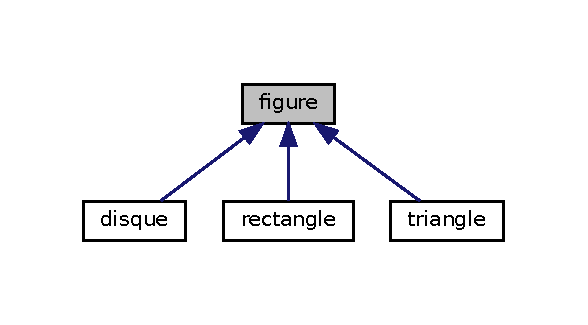
\includegraphics[width=282pt]{classfigure__inherit__graph}
\end{center}
\end{figure}
\subsection*{Public Member Functions}
\begin{DoxyCompactItemize}
\item 
\mbox{\Hypertarget{classfigure_a6ad51de31732e21f412ee7482e688ed0}\label{classfigure_a6ad51de31732e21f412ee7482e688ed0}} 
int {\bfseries perimetre} ()
\item 
\mbox{\Hypertarget{classfigure_a28b97e5819bec4048e69ecfe8a19043a}\label{classfigure_a28b97e5819bec4048e69ecfe8a19043a}} 
int {\bfseries aire} ()
\end{DoxyCompactItemize}


\subsection{Detailed Description}
\textbackslash{} Fichier \hyperlink{figure_8h_source}{figure.\+h} \textbackslash{} Appelle les fonctions des fichiers rectangle.\+cpp/rectangle.cpp/triangle.\+cpp \textbackslash{} Auteur Rayhan \textbackslash{} Version 1

\textbackslash{} Class figure \textbackslash{} Utilise l\textquotesingle{}héritage, la class appelera les fonctions dans les fichiers.\+cpp qui détiennent les fonctions perimetre/air. \textbackslash{} Fonction a \+: fonction perimetre, utilise les paramètres et codes des fichiers.\+cpp appelés \textbackslash{} Fonction b \+: fonction air, pareil que pour la fonction perimetre mais avec l\textquotesingle{}air \textbackslash{} Retourne donc les calcules de l\textquotesingle{}air et perimetre de l\textquotesingle{}objet demandé 

The documentation for this class was generated from the following file\+:\begin{DoxyCompactItemize}
\item 
/home/seance3/src/figure.\+h\end{DoxyCompactItemize}

\hypertarget{classrectangle}{}\section{rectangle Class Reference}
\label{classrectangle}\index{rectangle@{rectangle}}


{\ttfamily \#include $<$rectangle.\+h$>$}



Inheritance diagram for rectangle\+:
\nopagebreak
\begin{figure}[H]
\begin{center}
\leavevmode
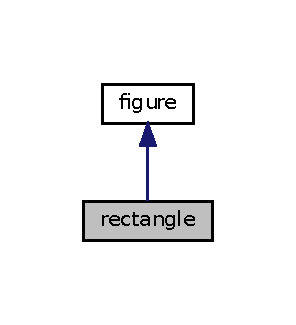
\includegraphics[width=142pt]{classrectangle__inherit__graph}
\end{center}
\end{figure}


Collaboration diagram for rectangle\+:
\nopagebreak
\begin{figure}[H]
\begin{center}
\leavevmode
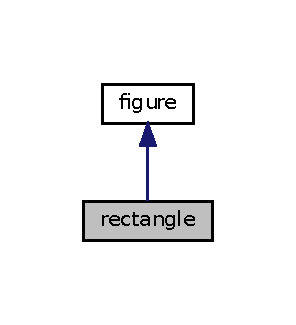
\includegraphics[width=142pt]{classrectangle__coll__graph}
\end{center}
\end{figure}
\subsection*{Public Member Functions}
\begin{DoxyCompactItemize}
\item 
int \hyperlink{classrectangle_a6de6e798ba0de4ca940ec2089a3bd774}{perimetre} (double cote1, double cote2)
\item 
int \hyperlink{classrectangle_ac96948e7667ebe186603b671d373f449}{aire} (double base, double hauteur)
\end{DoxyCompactItemize}


\subsection{Detailed Description}
\textbackslash{} Fichier \hyperlink{rectangle_8h_source}{rectangle.\+h} \textbackslash{} Appelle les fonctions du fichier rectangle.\+cpp \textbackslash{} Auteur Rayhan \textbackslash{} Version 1

\textbackslash{} Class rectangle \textbackslash{} Classe qui permet de calculer le perimetre ou l\textquotesingle{}aire d\textquotesingle{}un rectangle \textbackslash{} Retourne les calcules de l\textquotesingle{}air et du perimetre d\textquotesingle{}un rectangle 

\subsection{Member Function Documentation}
\mbox{\Hypertarget{classrectangle_ac96948e7667ebe186603b671d373f449}\label{classrectangle_ac96948e7667ebe186603b671d373f449}} 
\index{rectangle@{rectangle}!aire@{aire}}
\index{aire@{aire}!rectangle@{rectangle}}
\subsubsection{\texorpdfstring{aire()}{aire()}}
{\footnotesize\ttfamily int rectangle\+::aire (\begin{DoxyParamCaption}\item[{double}]{base,  }\item[{double}]{hauteur }\end{DoxyParamCaption})}

\textbackslash{} Fonction aire pour calculer l\textquotesingle{}aire du retangle \textbackslash{} parametre a \+: base du triangle \textbackslash{} parametre b \+: hauteur du triangle \textbackslash{} retourne le calcule ((base$\ast$hauteur)\%2) \mbox{\Hypertarget{classrectangle_a6de6e798ba0de4ca940ec2089a3bd774}\label{classrectangle_a6de6e798ba0de4ca940ec2089a3bd774}} 
\index{rectangle@{rectangle}!perimetre@{perimetre}}
\index{perimetre@{perimetre}!rectangle@{rectangle}}
\subsubsection{\texorpdfstring{perimetre()}{perimetre()}}
{\footnotesize\ttfamily int rectangle\+::perimetre (\begin{DoxyParamCaption}\item[{double}]{cote1,  }\item[{double}]{cote2 }\end{DoxyParamCaption})}

\textbackslash{} Fonction perimetre pour calculer le perimetre du rectangle \textbackslash{} parametre a \+: cote1 sur la longueur \textbackslash{} parametre b \+: cote2 sur la largeur \textbackslash{} retourne le calcul ((cote1+cote2)$\ast$2) 

The documentation for this class was generated from the following files\+:\begin{DoxyCompactItemize}
\item 
/home/seance3/src/figure.\+cpp\item 
/home/seance3/src/rectangle.\+h\item 
/home/seance3/src/rectangle.\+cpp\end{DoxyCompactItemize}

\hypertarget{classtriangle}{}\section{triangle Class Reference}
\label{classtriangle}\index{triangle@{triangle}}


{\ttfamily \#include $<$triangle.\+h$>$}



Inheritance diagram for triangle\+:
\nopagebreak
\begin{figure}[H]
\begin{center}
\leavevmode
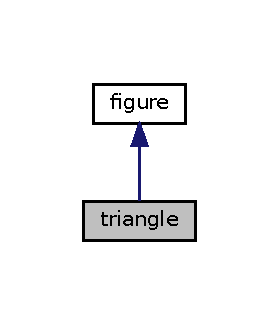
\includegraphics[width=134pt]{classtriangle__inherit__graph}
\end{center}
\end{figure}


Collaboration diagram for triangle\+:
\nopagebreak
\begin{figure}[H]
\begin{center}
\leavevmode
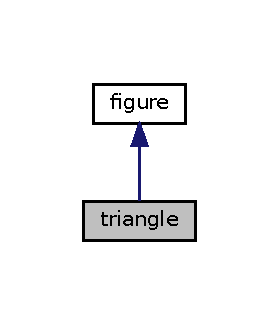
\includegraphics[width=134pt]{classtriangle__coll__graph}
\end{center}
\end{figure}
\subsection*{Public Member Functions}
\begin{DoxyCompactItemize}
\item 
int \hyperlink{classtriangle_a82bfb1d9a931d224519e5970f0dc438f}{perimetre} (double cote1, double cote2, double cote3)
\item 
int \hyperlink{classtriangle_a8683b3301b318f00d2a097541d81c8a7}{aire} (double base, double hauteur)
\end{DoxyCompactItemize}


\subsection{Detailed Description}
\textbackslash{} Fichier \hyperlink{triangle_8h_source}{triangle.\+h} \textbackslash{} Appelle les variables du fichier triangle.\+cpp \textbackslash{} Auteur Rayhan \textbackslash{} Version 1

\textbackslash{} Class triangle \textbackslash{} Permet de calculer l\textquotesingle{}aire et le perimetre d\textquotesingle{}un triangle \textbackslash{} Retourne les cacules de l\textquotesingle{}air et du perimetre d\textquotesingle{}un triangle 

\subsection{Member Function Documentation}
\mbox{\Hypertarget{classtriangle_a8683b3301b318f00d2a097541d81c8a7}\label{classtriangle_a8683b3301b318f00d2a097541d81c8a7}} 
\index{triangle@{triangle}!aire@{aire}}
\index{aire@{aire}!triangle@{triangle}}
\subsubsection{\texorpdfstring{aire()}{aire()}}
{\footnotesize\ttfamily int triangle\+::aire (\begin{DoxyParamCaption}\item[{double}]{base,  }\item[{double}]{hauteur }\end{DoxyParamCaption})}

\textbackslash{} Permet de calculer l\textquotesingle{}aire \textbackslash{} parametre a \+: base du triangle \textbackslash{} parametre b \+: hauteur du triangle \textbackslash{} retourne le calcule ((base$\ast$hauteur)\%2) \mbox{\Hypertarget{classtriangle_a82bfb1d9a931d224519e5970f0dc438f}\label{classtriangle_a82bfb1d9a931d224519e5970f0dc438f}} 
\index{triangle@{triangle}!perimetre@{perimetre}}
\index{perimetre@{perimetre}!triangle@{triangle}}
\subsubsection{\texorpdfstring{perimetre()}{perimetre()}}
{\footnotesize\ttfamily int triangle\+::perimetre (\begin{DoxyParamCaption}\item[{double}]{cote1,  }\item[{double}]{cote2,  }\item[{double}]{cote3 }\end{DoxyParamCaption})}

\textbackslash{} Permet de calculer le perimetre \textbackslash{} parametre a \+: côté 1 du triangle \textbackslash{} parametre b \+: côté 2 du triangle \textbackslash{} parametre c \+: côté 3 du triangle \textbackslash{} retourne le calcul (cote1+cote2+cote3) 

The documentation for this class was generated from the following files\+:\begin{DoxyCompactItemize}
\item 
/home/seance3/src/figure.\+cpp\item 
/home/seance3/src/triangle.\+h\item 
/home/seance3/src/triangle.\+cpp\end{DoxyCompactItemize}

%--- End generated contents ---

% Index
\backmatter
\newpage
\phantomsection
\clearemptydoublepage
\addcontentsline{toc}{chapter}{Index}
\printindex

\end{document}
